\pdfoutput=1
\documentclass[article,aps,nofootinbib,twocolumn,superscriptaddress]{revtex4-1}
\input epsf
\usepackage{graphics}
\usepackage{amsmath}
\usepackage{amssymb}
\usepackage{bm}
\usepackage{braket}
\usepackage{booktabs}
\usepackage{subfigure}
\usepackage{subfloat}
\usepackage{float}
\usepackage[usenames,svgnames]{xcolor}
\usepackage{hyperref}

\hypersetup{
    colorlinks=true,
    urlcolor=SteelBlue,
    linkcolor=red,
    citecolor=blue,
}


\usepackage{color}
\usepackage{dcolumn}
\usepackage{hyphenat}


\def\be{\begin{equation}}
\def\ee{\end{equation}}
\def\ba{\begin{eqnarray}}
\def\ea{\end{eqnarray}}

\newcommand{\ack}[1]{[{\bf Pfft!#1}]}
\newcommand{\tvb}[1]{{\bf \color{blue}{{#1}}}}
\newcommand{\tvg}[1]{{\bf \color{green}{{#1}}}}
\newcommand{\tvr}[1]{{\bf \color{red}{{#1}}}}
\newcommand{\ay}[1]{{\bf \color{magenta}{{#1}}}}

%\maketitle
\usepackage{graphicx}

\begin{document}

\title{Echoes from the scattering of wavepackets on wormholes}

\author{Jos\'e T. G\'alvez Ghersi}
\email{joseg@sfu.ca}
\author{Andrei V. Frolov}
\email{frolov@sfu.ca}
\author{David Dobre}
\email{ddobre@sfu.ca}
\affiliation{Department of Physics, Simon Fraser University, Burnaby, BC, V5A 1S6, Canada}


\begin{abstract}
In the light of the recent progress showing that the hypothetical observation of pulses isolated from the gravitational radiation transient (also known as echoes) would prove the existence of exotic compact objects (ECOs); it is possible to reproduce many features of the ringdown signal by simulating a scattering problem instead of the full coalescence of ECOs. In this paper, we study the dynamics of scalar and tensor wavepackets colliding against a spherically symmetric traversable wormhole. Our purpose is to extract the features of the time-dependent scattering solutions inside and outside the effective potential cavity in addition to their asymptotic behavior. Using the geometrical optics approximation, we show that the amplitude of the echoes is only large enough in a narrow bandwidth of frequency space, where the intensity of the transient reduces. The computer code used to produce these results is publicly available for further applications, including scattering and accretion processes.      
\end{abstract}

\maketitle


\section{Introduction}
The era of gravitational wave (GW) astronomy \citep{Abbott:2016blz, Abbott:2016nmj} has begun. GW spectroscopy, in contrast to its atomic counterpart, allows us to characterize strong gravitational interactions in their radiative regime. In this new range of frequencies, it is now possible to explore the role of dynamical gravitational degrees of freedom in a wide range of astrophysical \citep{Frolov:2017asg, Cardoso:2016rao} and cosmological \citep{Krauss989, Ade:2018gkx} phenomena. 

The prolonged absence of observational evidence confirming the dynamical properties of spacetime has motivated a plethora of conjectures about the behaviour of gravity within and beyond \citep{Clifton:2011jh, Taliotis:2012sx, Joyce:2014kja} classical General Relativity (GR). Latterly, the potential existence of exotic compact objects (ECOs) sourced by quantum effects on gravity \citep{PhysRevLett.61.1446, Almheiri:2012rt, Mazur:2001fv} (such as wormholes, firewalls and gravastars) has captured the attention of many recent efforts \citep{Cardoso:2016oxy, Abedi:2016hgu, Abedi:2018npz}. Wherein the primary claim is that the detection of a train of ``echoes'' isolated from the main transient of GW and with generically large amplitudes would be clear evidence of ECOs. It is, therefore, necessary to understand (i) the mechanisms behind the production of echoes and (ii) the intensity and spectrum of the outgoing wavelets compared to the GW transient in the most straightforward possible setup. In this paper, we explore the generation of echoes by colliding wavepackets of scalar and tensor radiation against a traversable spherically symmetric wormhole \citep{Visser:1989kh}. Such a wormhole behaves just like a Fabry-Perot cavity, shares common properties with the effective potential cavities made by other ECOs, like gravastars and firewalls, and the main features of the dispersed pulses are similar to the ringdown signals after the coalescence of ECOs.

Here we consider a wormhole configuration made by the junction of two Schwarzschild geometries of equal masses at $r_0>2M$, just as shown in \citep{Cardoso:2016oxy}. In this case, the symmetry of the centrifugal barriers at $r=3M$ on each side of the throat allows us to find the reflection and transmission coefficients of the cavity. Hence, it is possible to reconstruct the spectral shape of the outgoing pulse using the geometrical optics approximation. Nevertheless, this approximation predicts an exponential decay of the subsequent higher order reflections, which appears instead as a power law in the full solution of the scattering problem. Thus, the excitation of quasinormal modes (QNMs) is the only cause for the presence of echoes in the time evolving profile, these modes are sourced by a sequence of internal reflections inside the potential cavity and then propagate throughout the surface of the maximal potential energy spheres (i.e., the ``edges'' of the potential barriers), while leaking energy into the exterior. QNMs of the Schwarzschild solution have been extensively studied and reproduced in various analytic and numerical simulations \citep{Chandrasekhar:1975zza, PhysRevD.46.4179}; thus it is easy to identify their characteristic frequencies in the spectrum of outgoing pulses. We as well present the full scattering solution both inside and outside the wormhole cavity in detail, along with the energy fluxes and the asymptotic solutions for the principal spherical modes of a scalar (and tensor) wavepackets. In addition to this, we find the width and frequency intervals contained in the incident wavepackets for which the outgoing the wavelets have maximal amplitudes. Our computer code is optimized to solve both scalar accretion and scattering problems and is publicly available in \url{https://github.com/andrei-v-frolov/accretion/tree/wormhole}.

The layout for this paper is as follows: in section \ref{sec:scalar}, we review the scattering problem of scalar waves starting by a quick overview of the dispersion of a Gaussian pulse by a Schwarzschild black hole. In this review, we will be able to calculate the transmission and reflection coefficients of the centrifugal barriers constituting the walls of the resonant cavity in the case of the wormhole. Our results show a frequency ``sweet spot'' such that the incident pulse is not fully reflected nor fully transmitted by the cavity, favouring multiple internal reflections that source the QNMs.  Furthermore, we solve the scattering problem by a wormhole directly using the same ingoing Gaussian wavepacket, and then we compare the Fourier transform of this solution with the pulse reconstructed following the geometrical optics approximation. We find that the approximate reconstruction matches the full solution, up to the peaks due to the QNM frequencies. Likewise, we evaluate the amplitude of each of the echoes as a function of the width of the initial gaussian waveform, finding that a single width of the incident pulse maximizes the amplitude of each echo. In section \ref{sec:tensor}, we extend all the results in the previous section for a Gaussian pulse of tensor fluctuations of the metric by following the even and odd decomposition of the tensor modes introduced by Regge, Wheeler and Zerilli in \citep{Regge:1957td, PhysRevD.2.2141, PhysRevD.5.2419, PhysRevD.5.2439}. Our results can be recasted in terms of the usual asymptotic polarization modes $h_+$ and $h_{\times}$, known as the perturbations of a flat metric. Finally, in section \ref{sec:conclusions}, we discuss and conclude.

\section{Scattering of scalar wavepackets}\label{sec:scalar}
In this section, we solve the scattering of a Gaussian wavepacket by a spherically symmetric wormhole. To do so, we will first review the dispersion by the centrifugal barrier of a spherically symmetric black hole in order to find the properties of the potential cavity.
\subsection{Scattering by a Schwarzschild black hole}\label{subsec:bh} 
The dispersion of scalar waves by a Schwarzschild black hole has been thoroughly studied \citep{doi:10.1063/1.522949, Sanchez:1976xm, Sanchez:1977si, Sanchez:1977vz}, it is crucial for our purposes to provide the full solution since it contains all the information of the potential barriers constituting the effective potential in the case of a wormhole. The dynamics of the scattering problem is found by solving the equation of motion for a test scalar field
\begin{equation}
\Box\Phi=0,\label{eq:scalar_eq_mov} 
\end{equation}
where $\Box\equiv g^{\alpha\beta}\nabla_{\alpha}\nabla_{\beta}$ is the standard d'Alembertian in a curved background. Here $g_{\alpha\beta}$ is the metric tensor in a spherically symmetric Schwarzschild-like static spacetime
\begin{equation}
g_{\alpha\beta}=-f(r)\delta^t_{\alpha}\delta^t_{\beta}+\frac{1}{f(r)}\delta^r_{\alpha}\delta^r_{\beta}+r^2\left(\delta^{\theta}_{\alpha}\delta^{\theta}_{\beta}+\sin^2\theta\delta^{\phi}_{\alpha}\delta^{\phi}_{\beta}\right).
\label{eq:Schwarzschild}
\end{equation}
\begin{figure}[t]
\centering
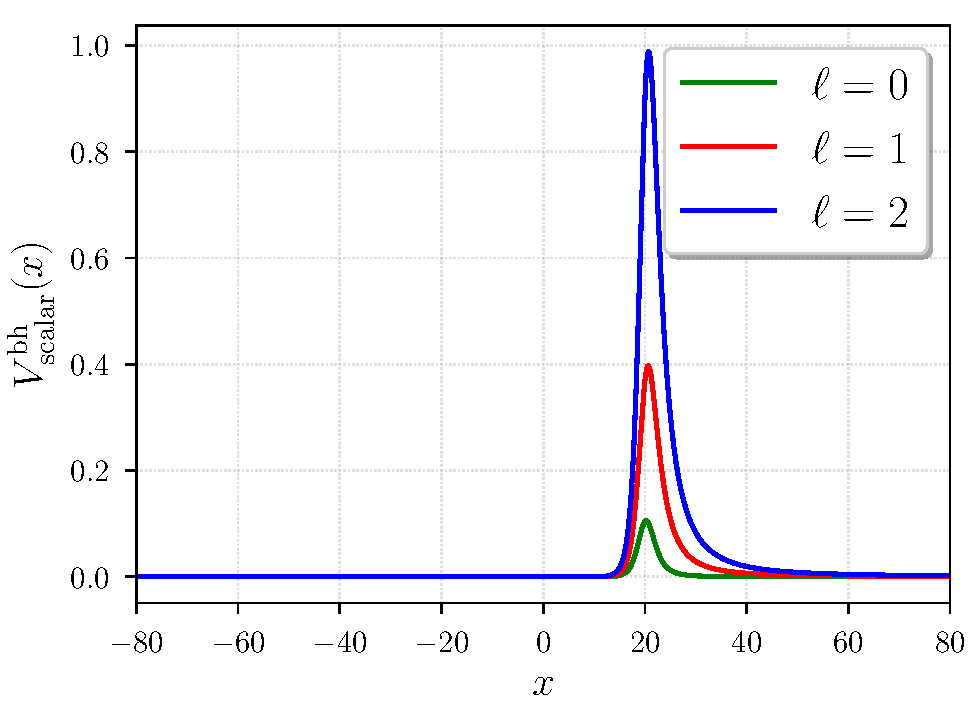
\includegraphics[width=.45\textwidth]{figures/potential_scalar_bh.pdf}
\caption{\label{fig:Potential_BH} Effective potential for the spherical modes $\mathcal{U}^{\mathrm{bh}}_{20}(x,t)$ scattered by a Schwarzschild black hole, growing with $\ell$. The wall acts as a barrier transparent to certain frequencies above a transmissivity threshold and reflective for lower frequencies.}
\end{figure}
It is convenient to introduce the tortoise coordinate $x$:
\begin{equation}
x\equiv\displaystyle{\int_{r_0}^r\frac{dr}{f(r)}},
\label{eq:tortoise}
\end{equation} 
In the case of the Schwarzschild metric $f(r)=1-r_g/r$ the last expression yields
\begin{equation}
x=r-r_0+r_g\ln\left(\frac{r-r_g}{r_0-r_g}\right),
\label{eq:tortoise2}
\end{equation} 
for $r_g<r<+\infty$ and $r_0>r_g$, where $r_g=2M$ is the usual Schwarzschild radius. By direct evaluation, we see that $r=r_0$ corresponds to $x=0$, the horizon $r=2M$ maps into $x\rightarrow-\infty$ and $r\rightarrow+\infty$ is $x\rightarrow+\infty$. In our numerical routine, we invert \eqref{eq:tortoise2} to get $r\equiv r(x)$ (see the appendix A, subsection 6 in \citep{Frolov:2017asg} for more details). In tortoise coordinates, we can decompose the scalar field in spherical harmonics 
\begin{equation}
\Phi(x,t)=\frac{1}{r(x)}\sum_{\ell,m=0}\mathcal{U}^{\mathrm{bh}}_{\ell m}(x,t)Y_{\ell m}(\theta,\phi),
\label{eq:ylm_decomp}
\end{equation}
in that way we can rewrite \eqref{eq:scalar_eq_mov} as
\begin{equation}
\left[-\partial_t^2+\partial_x^2-V_{\mathrm{scalar}}(x)\right]\mathcal{U}^{\mathrm{bh}}_{\ell m}(x,t) = 0,
\label{eq:wave_scalar}
\end{equation}
and the effective potential $V_{\mathrm{scalar}}(x)$ is given by
\begin{equation}
V_{\mathrm{scalar}}(x) = \left(1-\frac{r_g}{r(x)}\right)\left[\frac{\ell(\ell+1)}{r(x)^2}+\frac{r_g}{r(x)^3}\right].
\end{equation}
After rearranging the variables, the equation of motion of the spherical modes is now written in its traditional linear waveform. In Fig.~\ref{fig:Potential_BH}, we observe the growth of the potential barrier with the angular momentum number $\ell$. The potential wall does not vanish for the monopole ($\ell=0$) due to the extra term proportional to $r^{-3}$ appearing after the coordinate change, which replaces the radial damping in the original Schwarzschild coordinates $(t,r)$. Such a term becomes subdominant for all $\ell\geq 1$. Intuitively, it is reasonable to expect that the modes with frequency above a given threshold can cross the barrier, while reflecting the lower frequency modes. 

Now we setup the scattering problem for one of the spherical modes ($\mathcal{U}^{\mathrm{bh}}_{20}$, the quadrupole) with the following initial conditions corresponding to an ingoing Gaussian wavepacket 
\begin{equation}
\mathcal{U}^{\mathrm{bh}}_{20}(x,0)=\exp\left(\frac{(x-x_0)^2}{2\sigma^2}\right)~,~ \partial_t\mathcal{U}^{\mathrm{bh}}_{20}\bigg{|}_{t=0}=\partial_x \mathcal{U}^{\mathrm{bh}}_{20}(x,0),
\label{eq:scalar_init_cond}
\end{equation}

\begin{figure}[t!]
\centering
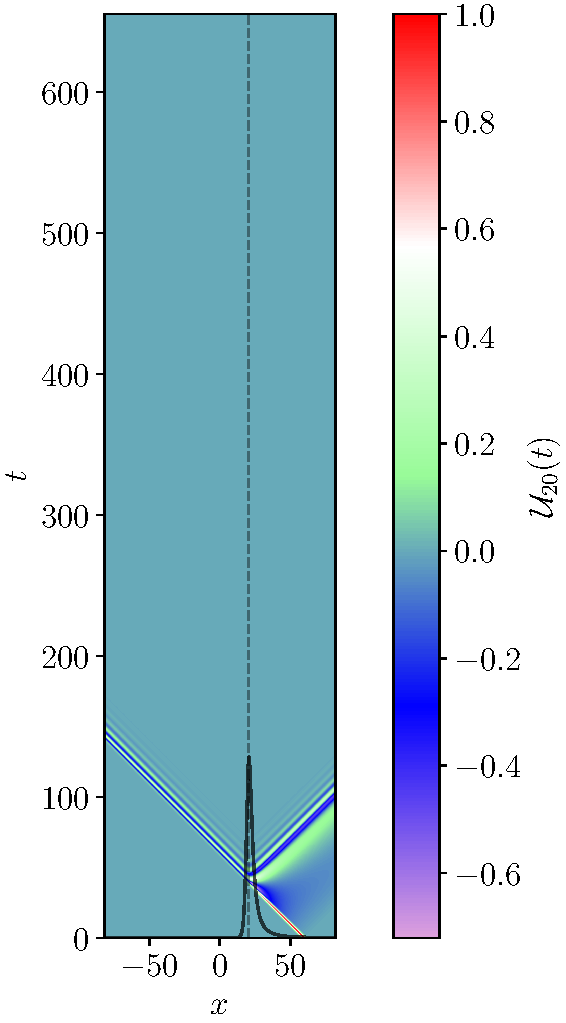
\includegraphics[width=.45\textwidth]{figures/bh_l_2.pdf}
\caption{\label{fig:bh_sol} Dispersion of the ingoing Gaussian wavepacket $\mathcal{U}^{\mathrm{bh}}_{20}$ by the potential barrier (plotted in black) showing the incident, reflected and transmitted pulses, it is possible notice the ringing of the reflected solution due to the quasinormal modes.}
\end{figure}

\begin{figure}[t]
\centering
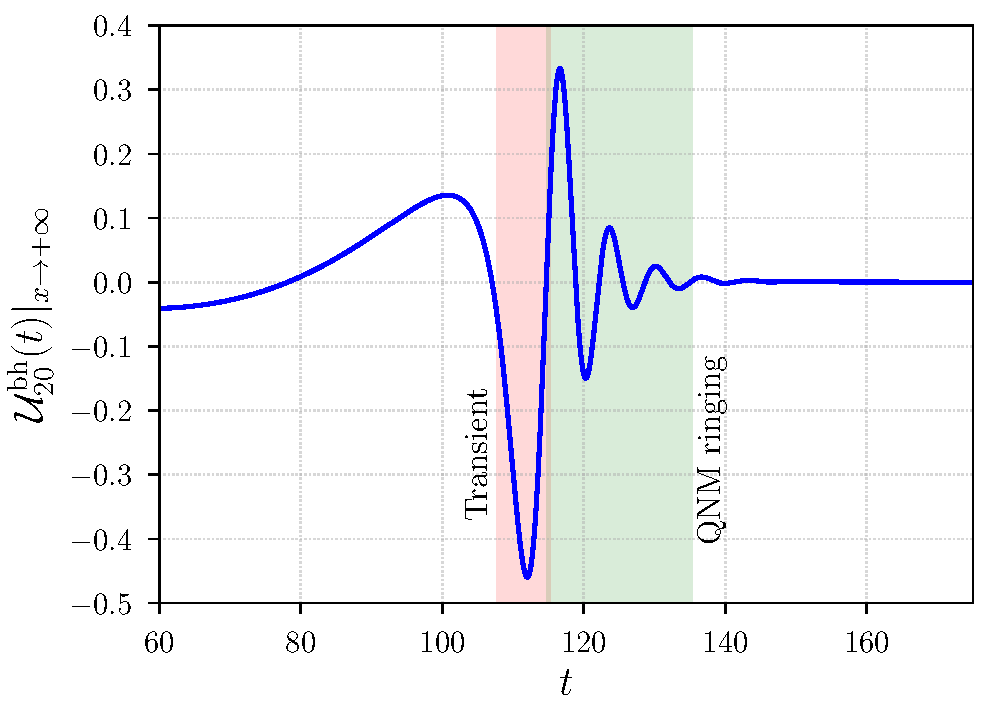
\includegraphics[width=.45\textwidth]{figures/Scalar_bh.pdf}
\caption{\label{fig:asympt_sol} Asymptotic solution for the quadrupole mode $\mathcal{U}^{\mathrm{bh}}_{20}(x,t)$ by direct evaluation of the results in Fig.~\ref{fig:bh_sol}. The reflected signal shows its maximum peak and the posterior ringing due to QNMs.}
\end{figure}

\begin{figure}[t]
\centering
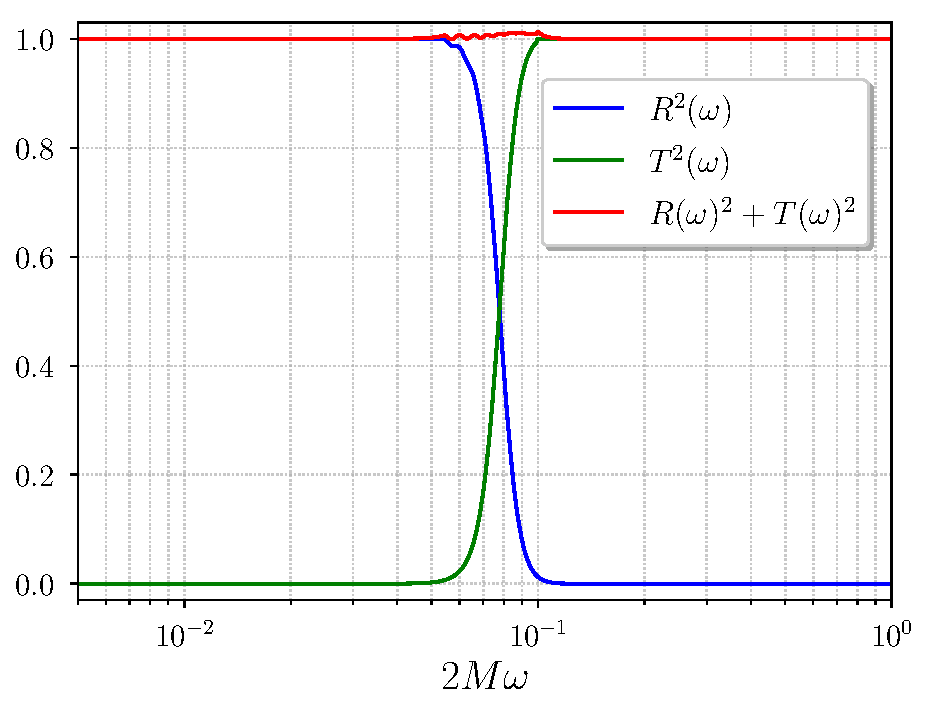
\includegraphics[width=.45\textwidth]{figures/RT_omega_scalar.pdf}
\caption{\label{fig:RT_scalar} Reflection and transmission coefficients as a function of frequency $(\omega)$, the identity $R^2+T^2=1$ is satisfied with an error smaller than 1\%.}
\end{figure}

After fixing the values of the width to be $\sigma=0.9185r_g$, the initial position of the Gaussian at $x_0=60.0r_g$, $r_0=20.0r_g$ and the initial conditions in \eqref{eq:scalar_init_cond}, we show the time-dependent solution of \eqref{eq:wave_scalar} in Fig.~\ref{fig:bh_sol}, where we distinguish the incident, transmitted and reflected parts of the solution. It is important to observe the absence of spurious late time reflections and interferences due to the implementation of perfectly matching layers (PMLs) in the outermost regions of our simulation box (see the details of our setup for PMLs in \citep{Frolov:2017asg}). We observe the main features of the reflected signal in Fig.~\ref{fig:asympt_sol}, where the asymptotic behavior of the signal shows a sharp transient is a consequence of the collision against the potential wall, and the ringing of quasinormal modes occurring right after the reflection in agreement with \citep{Petrich:1985csm}. 

It is now possible to evaluate the reflection and transmission coefficients of the potential wall depicted in Fig.~\ref{fig:Potential_BH}. To do so, we compute the one dimensional Fourier transform of the incident $\tilde{\mathcal{U}}_{20}^{\mathrm{inc}}(\omega)=\mathcal{F}[\mathcal{U}^{\mathrm{bh}}_{20}(0,x)]$, reflected $\tilde{\mathcal{U}}_{20}^{\mathrm{ref}}(\omega)=\mathcal{F}[\mathcal{U}^{\mathrm{bh}}_{20}(t,+\infty)]$ and transmitted $\tilde{\mathcal{U}}_{20}^{\mathrm{trans}}(\omega)=\mathcal{F}[\mathcal{U}^{\mathrm{bh}}_{20}(t,-\infty)]$ from the solved scattering modes in order to define
\begin{equation}
R(\omega)\equiv \frac{||\tilde{\mathcal{U}}_{20}^{\mathrm{ref}}(\omega)||}{||\tilde{\mathcal{U}}_{20}^{\mathrm{inc}}(\omega)||}~,~T(\omega)\equiv \frac{||\tilde{\mathcal{U}}_{20}^{\mathrm{trans}}(\omega)||}{||\tilde{\mathcal{U}}_{20}^{\mathrm{inc}}(\omega)||}
\label{eq:ref_and_trans}
\end{equation}
\begin{figure}[t]
\centering
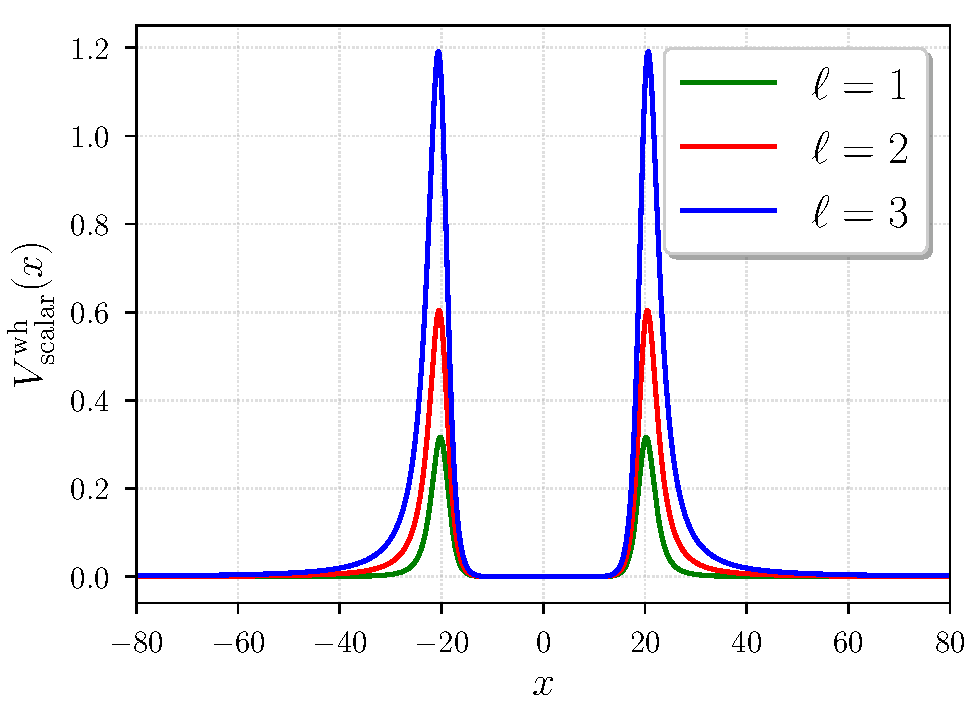
\includegraphics[width=.4\textwidth]{figures/potential_scalar.pdf}
\caption{\label{fig:potential_wh} Effective potential cavity for the wormhole, we observe the growth of the barriers with the angular momentum number $\ell$.}
\end{figure}

as the transmission and reflection coefficients, respectively. In Fig.~\ref{fig:RT_scalar}, we plot the squares of these coefficients as functions of frequency observing that the identity $R^2+T^2=1$ is only approximately met because of the small contributions coming from the QNMs frequency peaks in both the transmitted and reflected solutions. The shape of both the transmissivity and reflectivity curves is very similar to an hyperbolic tangent step function\footnote{This is not surprising after we consider the DeWitt approximation for the transmissivity \citep{DeWitt:1975ys,Frolov:1998wf}, which is precisely given by a step function.}, intersecting at $R^2=T^2=0.5$, as expected. Furthermore, it is crucial to notice from the last figure that it is only in a narrow band of frequencies where the amplitudes transmitted and reflected by the potential barrier are comparable. in the case of a wormhole, such a fact will be important in our analysis.  

\subsection{Scattering by a traversable wormhole}\label{subsec:wh} 
In this section, we study the dispersion of Gaussian wavepackets by a traversable wormhole, formed by the junction at $r_0>r_g$ of two Schwarzschild black hole solutions with equal mass. There is a discontinuity in $G_{\alpha\beta}$ such that at $r=r_0=20.0r_g$, any contracting congruence of geodesics in one side of the throat starts to expand in order to reach the other side, violating the weak energy condition.
The dynamics of the scattering problem is still given by the solutions of \eqref{eq:scalar_eq_mov} following the same decomposition in spherical modes as in \eqref{eq:ylm_decomp}. Hence, the waveform of the equation of motion for the spherical modes is given by
\begin{equation}
\left[-\partial_t^2+\partial_x^2-V^{\mathrm{wh}}_{\mathrm{scalar}}(x)\right]\mathcal{U}_{\ell m}(x,t) = 0,
\label{eq:wave_scalar_wh}
\end{equation}
and the effective potential $V^{\mathrm{wh}}_{\mathrm{scalar}}(x)$ yields
\begin{equation}
V^{\mathrm{wh}}_{\mathrm{scalar}}\left(x\right) = \left(1-\frac{r_g}{r\left(|x|\right)}\right)\left[\frac{\ell(\ell+1)}{r\left(|x|\right)^2}+\frac{r_g}{r\left(|x|\right)^3}\right].
\end{equation}   
\begin{figure}[t!]
\centering
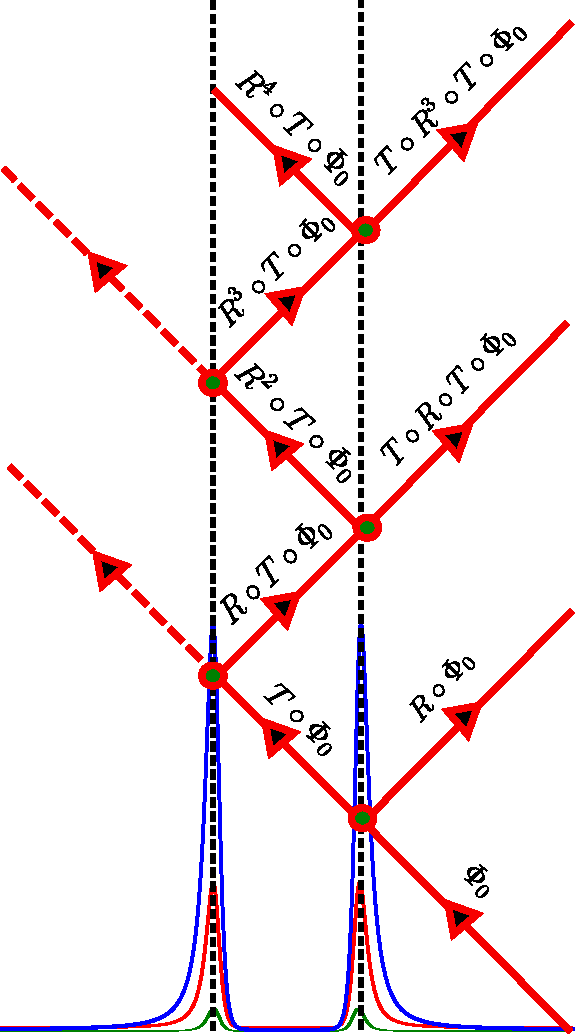
\includegraphics[width=.3\textwidth]{figures/Geom_optics.pdf}
\caption{\label{fig:Geom_optics} Schematic reconstruction of the outgoing solution by a sequence of reflections and transmissions inside the potential cavity.}
\end{figure}
which is plotted in Fig.~\ref{fig:potential_wh} and coincides with the shape of the potential calculated in \citep{Cardoso:2016oxy}. Strictly speaking, we refer to $r\left(|x|\right)$ as the same inverse of the function mentioned in \eqref{eq:tortoise2} now evaluated at $|x|-r_0$. As we can see in Fig.~\ref{fig:potential_wh}, the new effective potential is merely a reflection of the potential barrier in Fig.~\ref{fig:Potential_BH} about the ordinate axis; thus, it is sensible to identify this system as a potential cavity built from two potential barriers with the reflection and transmission coefficients depicted in Fig.~\ref{fig:RT_scalar}. Furthermore, let us assume that an arbitrary incident pulse $\Phi_0$ propagates towards the cavity, it is, therefore, reasonable to approximate the spectrum of the asymptotic solution by a simple geometrical series of reflections and transmissions inside the cavity acting on the incident pulse, as shown in Fig.~\ref{fig:Geom_optics}. Following this scheme, the asymptotic solution can be approximated by
\begin{equation}
\Phi^{\mathrm{wh}}(\omega)|_{x\rightarrow+\infty}=\left[R+T\circ\sum_{i=0}R^{2i+1}\circ T\right]\circ\Phi_0(\omega).
\label{eq:reconst}
\end{equation}
It is not difficult to see that, in the hypothetic case of a perfectly reflective wall replacing the left potential barrier in Figs.~\ref{fig:potential_wh} and \ref{fig:Geom_optics}, the reconstructed pulse is instead given by 
\begin{equation}
\Phi^{\mathrm{f}}(\omega)|_{x\rightarrow+\infty}=\left[R+T\circ\sum_{i=0}R^i\circ T\right]\circ\Phi_0(\omega),
\label{eq:reconst_firewall}
\end{equation}
corresponding to the case of a firewall. We will not cover the features of the firewall solution in what remains of this paper. 

\begin{figure*}
\centering
\subfigure{
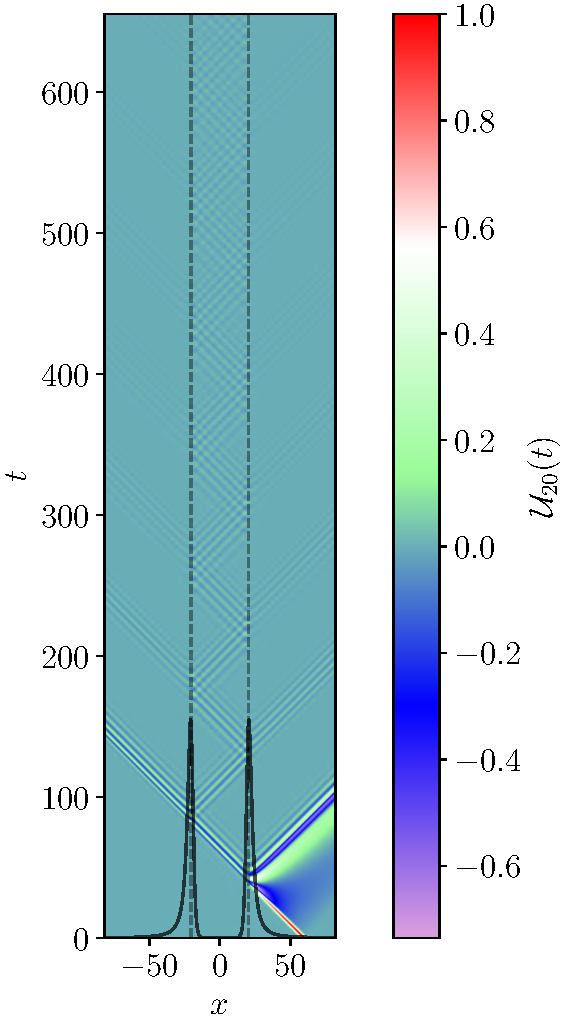
\includegraphics[width=.4\textwidth]{figures/wh_l_2.pdf}} \,
\subfigure{
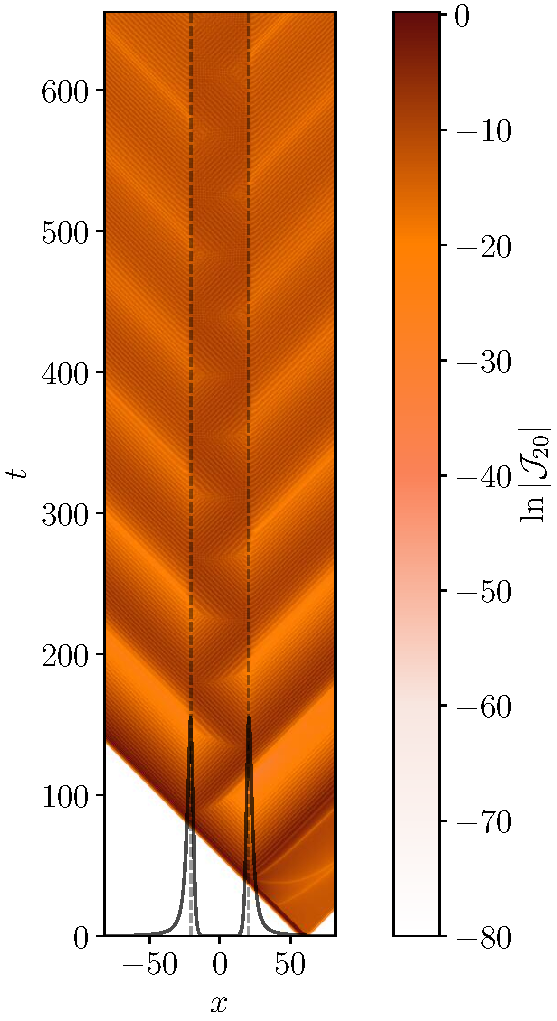
\includegraphics[width=.4\textwidth]{figures/wh_flux_l_2.pdf}}
\caption{\label{fig:sol_n_flux_wh} Left panel: Evolution of the quadrupole mode $\mathcal{U}_{20}$ for the effective potential in Fig.~\ref{fig:potential_wh}. We can notice the sequence of reflections and transmissions inside the cavity is very similar to the scheme depicted in Fig.~\ref{fig:Geom_optics}. Right panel: Evolution of the radial flux $\mathcal{J}_{20}\equiv \mathcal{U}_{20,x} \mathcal{U}_{20,t}$, the only incident source comes from the collision of the pulse, which dissipates very slowly to the exterior every time the internal reflections hit the walls of the potential cavity. QNM are sourced by this process.} 
\end{figure*}

We now solve the scattering problem exactly for the quadrupole mode $\mathcal{U}_{20}(t,x)$. Using the same initial conditions as in \eqref{eq:scalar_init_cond} for $\sigma=0.9185r_g$ as the width of the incident Gaussian pulse, we find the time-dependent solution of the quadrupole mode $\mathcal{U}_{20}$ (left panel) and its radial flux $\mathcal{J}_{20}\equiv \mathcal{U}_{20,x} \mathcal{U}_{20,t}$ (right panel) in Fig.~\ref{fig:sol_n_flux_wh}. It is interesting to notice in the evolution plot (on the left) that the signal forms an interference pattern at very late times, showing that this process might fill the cavity. In addition to this, even when the amplitude of the modes decreases after each collision against any of the potential walls, the spherical modes propagate for longer time throughout the spheres of maximal potential. 

The scalar flux is shown in the right panel, we observe that the only source of scalar radiation comes from the first collision of the Gaussian wavepacket against the barrier in the right hand side (the ingoing flux is colored in black at the bottom of the contour plot). A sequence of reflections occurs within the potential barriers, which decay in intensity with time as the cavity leaks energy to the exterior.

\begin{figure*}
\centering
\subfigure{
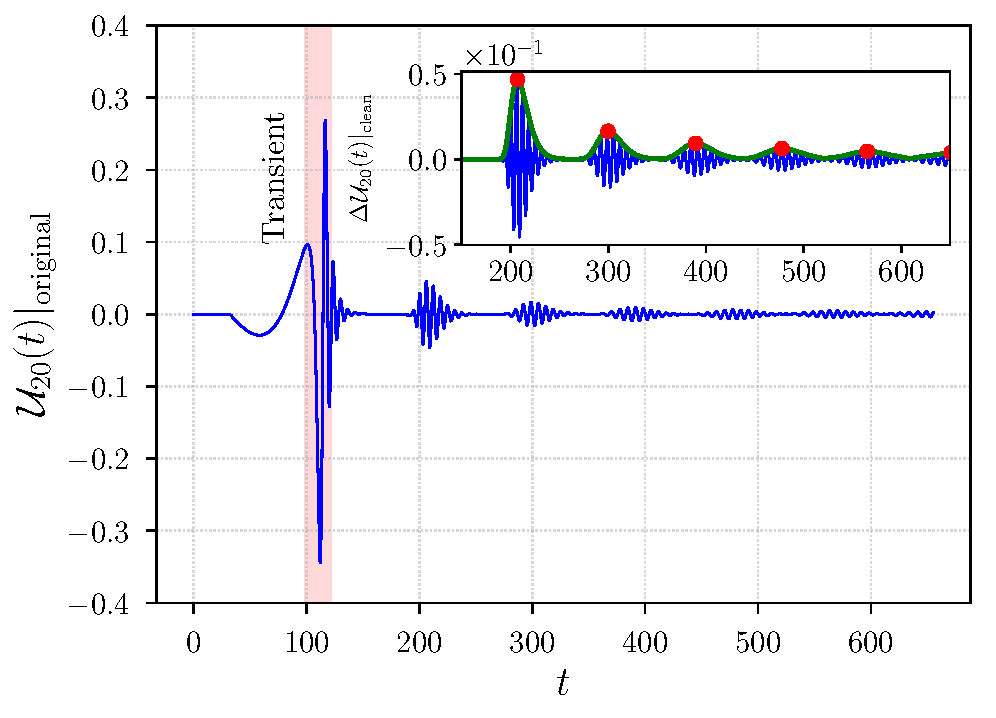
\includegraphics[width=.45\textwidth]{figures/Scalar_echo_w_06495.pdf}} \,
\subfigure{
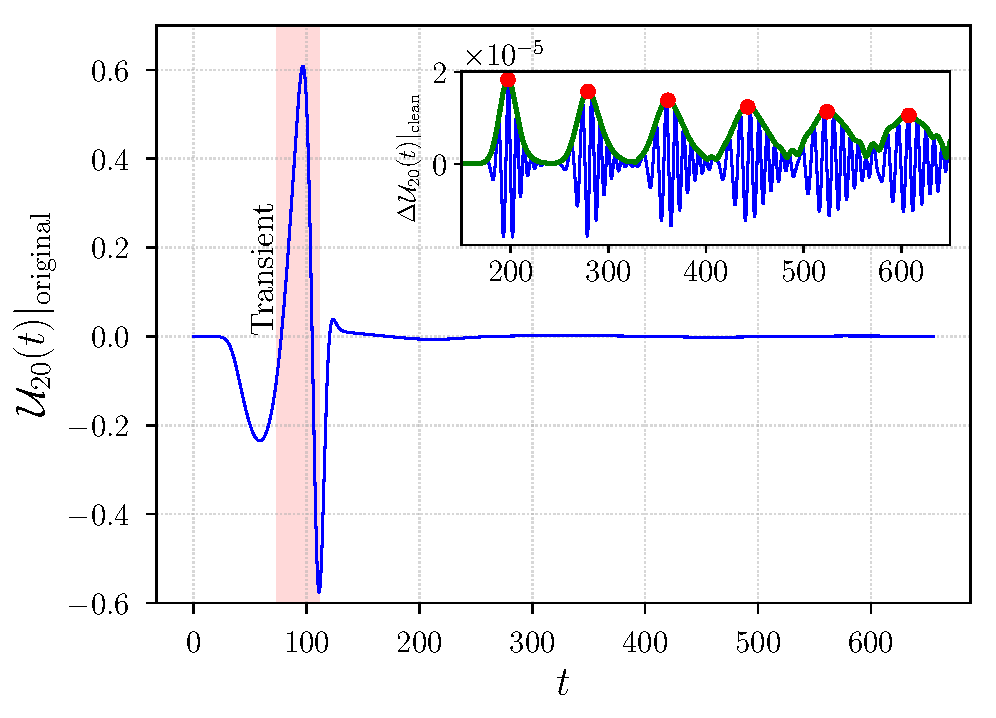
\includegraphics[width=.45\textwidth]{figures/Scalar_echo.pdf}}
\caption{\label{fig:asympt_two_sigmas} Left panel: Asymptotic evolution of the quadrupole mode $\mathcal{U}_{20}$ for $\sigma=0.6495r_g$. Echoes are plotted in the upper corner of the plot, showing them along with their Hilbert envelope (the curves in green) and maximum amplitudes (in red). Right panel: Asymptotic evolution of the quadrupole mode $\mathcal{U}_{20}$ for $\sigma=5.196r_g$. In contrast with the left panel, echoes are four orders of magnitude smaller than the transient. The amplitude of the transient in the right figure has decreased with respect to the one in the left panel.} 
\end{figure*}

The amplitude of the outgoing signals depends on the width of the incident Gaussian wavepacket, this is visible in Fig.~\ref{fig:asympt_two_sigmas} where we plot the asymptotic solutions for two different ingoing wavepackets: one with $\sigma=0.6495r_g$ in the left panel and a second one with $\sigma=5.196r_g$ in the right. After subtracting the outgoing solution for a black hole, the presence of a train of wavelets, widely known as echoes, is very clear. The signal is not a straight line after the transient, as we can observe in the right panel of this figure. Therefore, subtracting the black hole outgoing pulse (i.e., the case in which there is only one potential wall) turns to be a convenient way to clean the signal from back reflections due to the ``tails'' of the potential barrier, especially since in this case the echoes are four orders of magnitude smaller than the transient. In both panels, we plot the variable $\Delta\mathcal{U}_{20}|_{\mathrm{clean}}\equiv\mathcal{U}_{20}|_{\mathrm{original}}-\mathcal{U}^{\mathrm{bh}}_{20}$ in the right upper corner of the figures to represent the echoes and their net amplitude without backscattering effects.
 
As shown in subsection \ref{subsec:bh}, the curves of reflectivity and transmissivity determine the frequencies going through the barriers of the potential cavity: most of the power of an incident pulse with large $\sigma$ is in the low frequency domain, and therefore it will be reflected. Moreover, the cavity is transparent to high frequency signals, which are dominant in the pulses with small $\sigma$. In either of these extremal scenarios, QNMs cannot be sourced by internal reflections and thus, the amplitude of the echoes is not large in general.\\
 
\begin{figure}[t!]
\centering
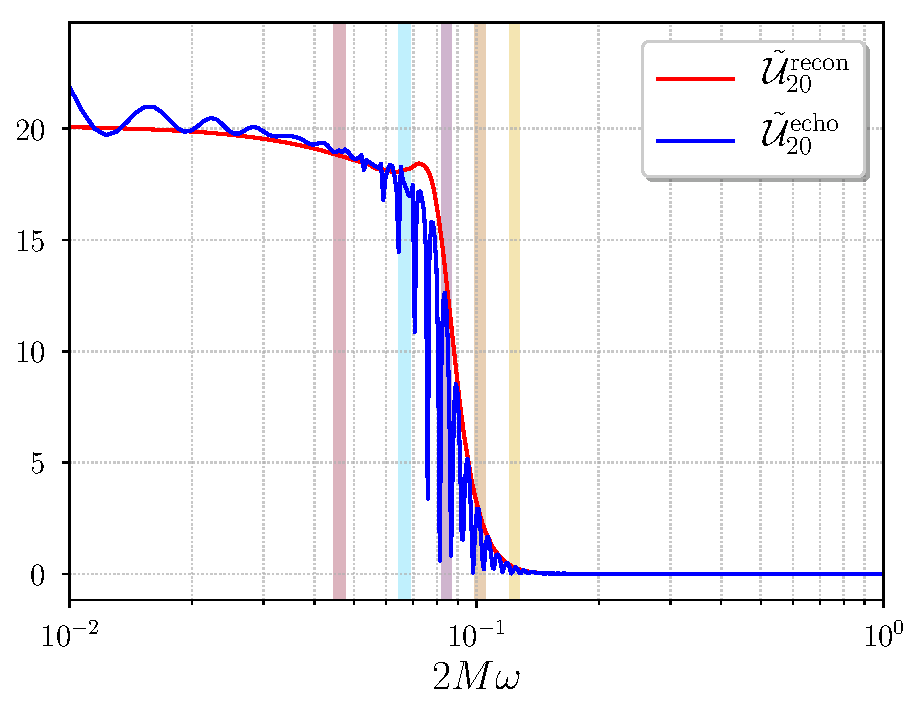
\includegraphics[width=.45\textwidth]{figures/Reconst_omega_scalar.pdf}
\caption{\label{fig:rec_scalar} Comparing the reconstruction of the spectrum by the geometrical optics approximation in \eqref{eq:reconst} (in red) with the Fourier transform of the full asymptotic solution $\tilde{\mathcal{U}}_{20}^{\mathrm{echo}}$ (in blue). The color stripes indicate a few of the first QNM frequency peaks corresponding to $\omega_3=0.251M^{-1}$ in golden rod, $\omega_4=0.207M^{-1}$ in peru, $\omega_5=0.169M^{-1}$ in plum, $\omega_6=0.133M^{-1}$ in light blue and $\omega_7=0.092M^{-1}$ in rosy brown, these are the real parts of the QNM frequencies for $n=3,4,5,6~\&~7$ calculated in \citep{PhysRevD.46.4179}.}
\end{figure} 

Now we proceed to reconstruct the asymptotic spectrum by following the geometrical optics relation in \eqref{eq:reconst} considering the reflectivity and transmissivity operators defined in \eqref{eq:ref_and_trans}. Then, the outcome should be compared with the spectral content of the asymptotic wave solutions of \eqref{eq:wave_scalar_wh}. We calculate the Fourier transforms of both the Gaussian incident pulse $\Phi_0(\omega)=\mathcal{F}[\exp\left((x-x_0)^2/2\sigma^2\right)]$ for $\sigma=0.6495r_g$ and $x_0=60.0r_g$, and the asymptotic solution $\tilde{\mathcal{U}}_{20}^{\mathrm{echo}}\equiv\mathcal{F}[\mathcal{U}_{20}(t,+\infty)]$, which includes the echoes.\\

\begin{figure*}
\centering
\subfigure{
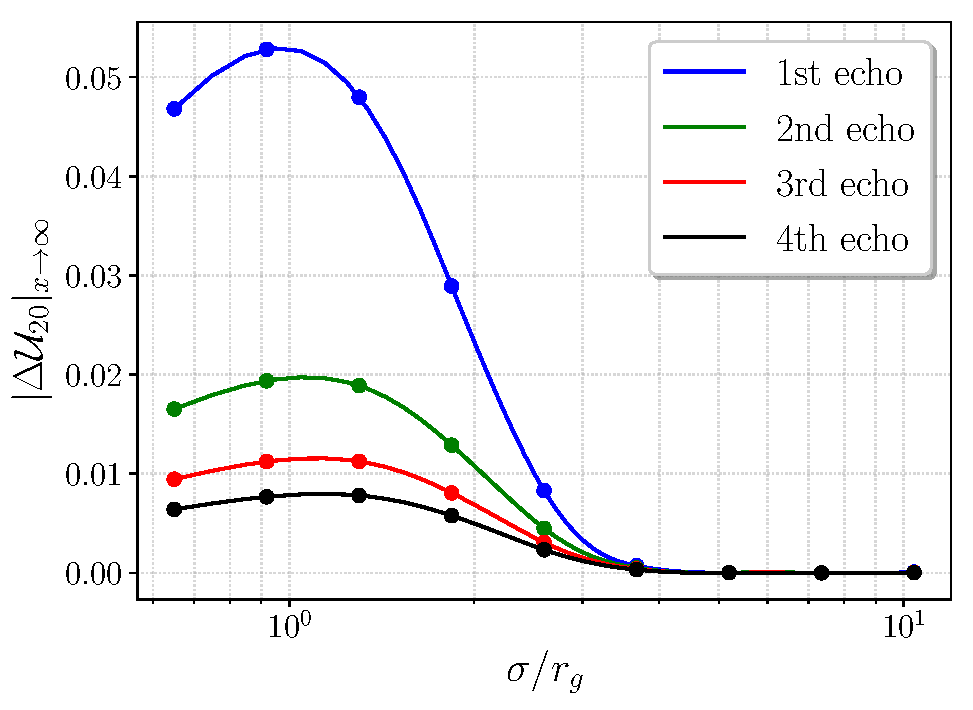
\includegraphics[width=.45\textwidth]{figures/Echo_sigma2_l_2.pdf}} \,
\subfigure{
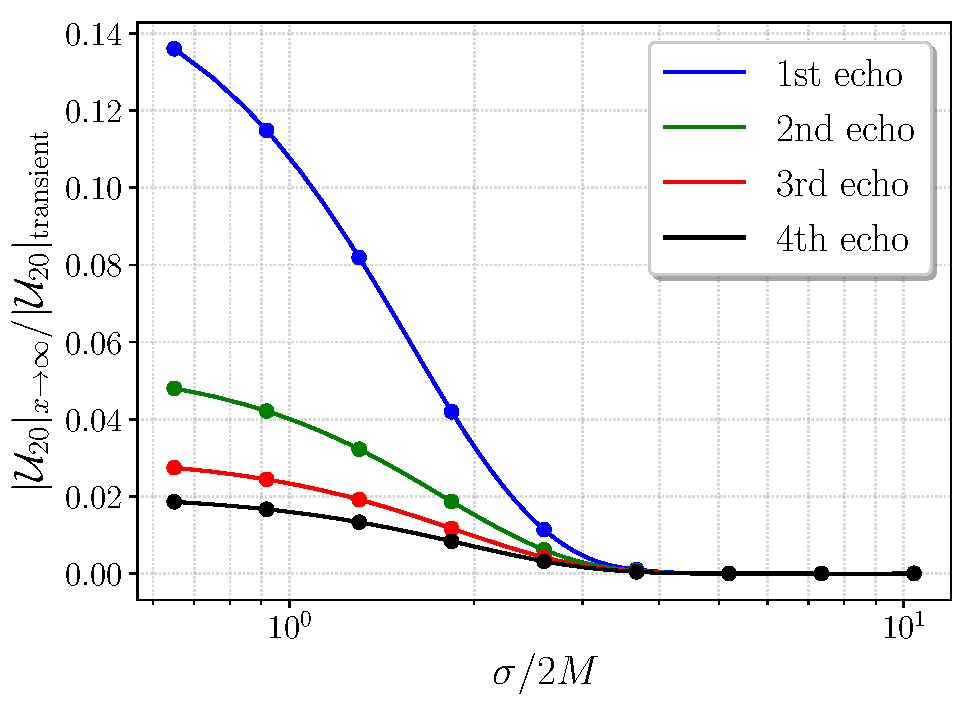
\includegraphics[width=.45\textwidth]{figures/Echo_sigma_l_2.pdf}}
\caption{\label{fig:echo_sigma} Left panel: Amplitudes of the first four echoes as a function of $\sigma$ for $\ell=2$, we observe the presence of a maximum amplitude of all the echoes at roughly $\sigma\approx r_g$, which is not incompatible with the de DeWitt approximation. Right panel: Relative amplitude of the first four echoes compared to the amplitude of the transient. The points represent the simulated wormhole/black hole pairs used in our analysis.} 
\end{figure*}

After applying the reconstruction expression in \eqref{eq:reconst} up to $i=0$ (in red), and comparing the outcome with $\tilde{\mathcal{U}}_{20}^{\mathrm{echo}}$, we show the reconstructed spectrum and $\tilde{\mathcal{U}}_{20}^{\mathrm{echo}}$ (in blue) in Fig.~\ref{fig:rec_scalar}. The low frequency oscillation peaks in the blue spectrum correspond to the finite size of the simulation box and should be ignored. Notice that the spectrum reconstructed employing the geometrical optics approximation gives the overall shape of the spectrum with decent precision but not the QNM frequency peaks, these appear in the same frequency interval where the reflectivity and transmissivity curves intersect in Fig.~\ref{fig:RT_scalar}. It is, therefore, reasonable to talk about a ``sweet spot'' in the frequency domain where the cavity maximizes the amplitude of the echoes. Intuitively, after observing the results in Fig.~\ref{fig:asympt_two_sigmas}, it is possible to identify a similar ``sweet spot'' in the parameter space space for the widths of the incident Gaussian wavepackets, considering this is a one parameter problem. However, it is also necessary to not only compare the amplitude of each individual echo with $\sigma$, but also the ratio between the amplitude of the echo with the amplitude of the transient for each value of the width, which is relevant since we are finding the relative intensity of the echoes compared to the strongest outgoing signal. 

To do so, we proceed as follows: we setup a logarithmic 1D grid of widths centered at $\sigma_{\mathrm{DW}}=\sqrt{27}r_g/2\ell$ --  the width of maximum transmissivity according to the DeWitt approximation \citep{DeWitt:1975ys} -- and spaced by increments of $\sqrt{2}\sigma_{\mathrm{DW}}$. Then, we find the amplitudes of the first four echoes for every width of the incident pulse without altering the properties of the cavity. In order to determine the amplitudes of the echoes, we need to subtract the reflection coming from the scattering of a single barrier (i.e., the black hole case) by using the variable $\Delta\mathcal{U}_{20}|_{\mathrm{clean}}\equiv\mathcal{U}_{20}|_{\mathrm{original}}-\mathcal{U}^{\mathrm{bh}}_{20}$. This requires a non-trivial computational effort since each scattering scenario needs to be solved twice (one for the wormhole and one for the black hole) in order to clean up the signal and obtain a clear view of the echoes. Once the signal is refined, we find its Hilbert transform \citep{1449626} in order to find its continuous envelope, which are the green curves in the upper corners of Fig.~\ref{fig:asympt_two_sigmas}, and therefore, the amplitudes of the echoes are the local maxima of their envelopes (the red dots in the same figure). 

We show our results in Fig.~\ref{fig:echo_sigma}, where we notice in the left panel the presence of a well-defined maximal amplitude of the first four echoes. This is consistent with the idea of a range of frequencies/widths that maximize the amplitudes of the echoes, as we shown in the analysis of the reflection and transmission coefficients: the cavity is transparent for small widths of the ingoing Gaussian (large frequencies) and is reflective for wide incident pulses. In the right panel, we observe the growth of the relative amplitude as the widths become smaller. Such a fact only means that the reduction of the transient is faster than the reduction of the echoes as the frequencies grow, as the cavity becomes more transparent the ingoing pulses get transmitted more efficiently. Therefore, this analysis is useful to get a basic understanding of the frequency/width scales in which echoes could be observable.  

\section{Scattering of tensor wavepackets}\label{sec:tensor} 
Following the perspective of the even/odd parity decomposition for tensor perturbations of a spherically symmetric spacetime \citep{Regge:1957td, PhysRevD.2.2141, PhysRevD.5.2419}, we implement all the techniques used in section \ref{sec:scalar} and extend our analysis to study the scattering of a test Gaussian wavepacket of tensor perturbations. From now on, we will follow the conventions in \citep{Martel:2005ir}, including the choice of the Regge-Wheeler gauge. 
The dynamics of the wave scattering problem is given by two equations of motion of the form
\begin{equation}
\left(\tilde{\Box}-\mathcal{V}_{\mathrm{eff}}\right)\Psi_{\ell m}=0,
\label{eq:tensor_eq_mov}
\end{equation} 
here $\tilde{\Box}\equiv g^{ab}\nabla_a\nabla_b$ is the 2D d'Alembertian operator in the usual $(a,b)\rightarrow(t,r)$ Schwarzschild coordinates. $\mathcal{V}_{\mathrm{eff}}$ corresponds one of two possible potentials, the Regge-wheeler (odd) potential, $\mathcal{V}_{\mathrm{odd}}$ 
\begin{equation}
\mathcal{V}_{\mathrm{odd}}(r)= \frac{\ell(\ell+1)}{r^2}-\frac{3r_g}{r^3},
\label{eq:V_odd}
\end{equation} 
\begin{figure*}
\centering
\subfigure{
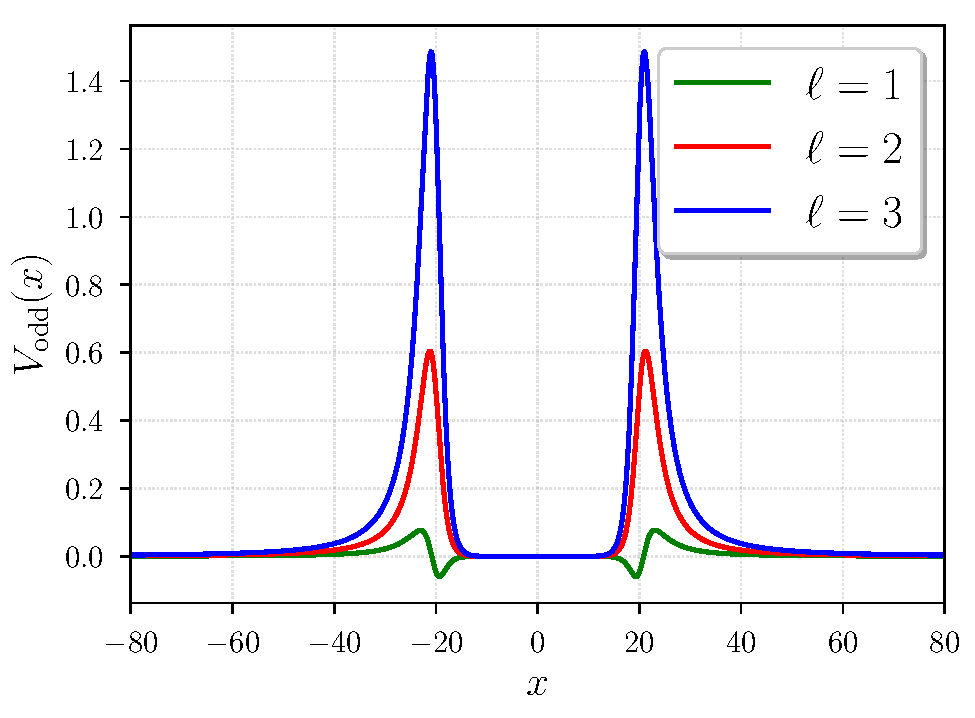
\includegraphics[width=.45\textwidth]{figures/potential_odd.pdf}} \,
\subfigure{
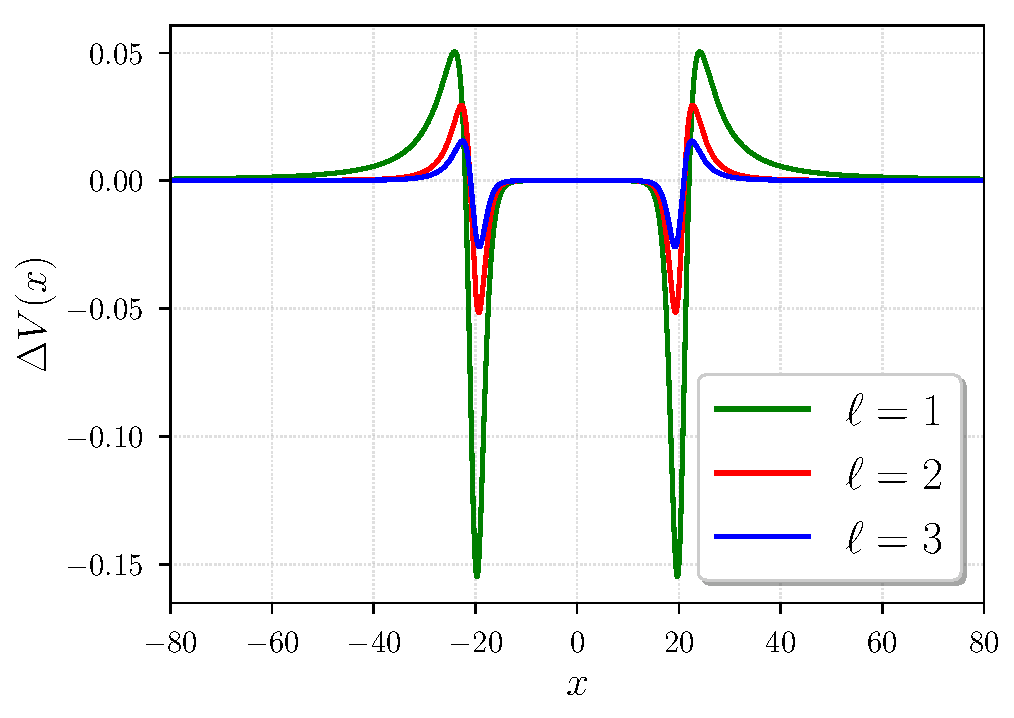
\includegraphics[width=.45\textwidth]{figures/delta_even_odd.pdf}} 
\caption{\label{fig:evenodd_potentials} Left panel: Plot of the Regge-Wheeler potential ($V_{\mathrm{odd}}\equiv[1-r_g/r(|x|)]\mathcal{V}_{\mathrm{odd}}$) as a function of the tortoise coordinate $x$. Right panel: Difference between the Regge-Wheeler and Zerilli effective potentials $\Delta V=V_{\mathrm{odd}}-V_{\mathrm{even}}$. The difference of the two potentials is below the order of 1\% for ($\ell\geq 2$).} 
\end{figure*}
or the Zerilli (even) potential, $\mathcal{V}_{\mathrm{even}}$ 
\begin{equation}
\mathcal{V}_{\mathrm{even}}(r)=\displaystyle{\frac{1}{\Lambda^2}\bigg[\mu^2\bigg(\frac{\mu+2}{r^2}+\frac{3r_g}{r^3}\bigg)+\frac{9r_g^2}{r^4}\left(\mu+\frac{r_g}{r}\right)\bigg]},
\label{eq:V_even}
\end{equation} 
where $\mu\equiv(\ell-1)(\ell+2)$ and $\Lambda\equiv\mu+3r_g/r$. All the source terms in proportional to the stress energy tensor and its contractions appearing in the right hand side of \eqref{eq:tensor_eq_mov} in \citep{Martel:2005ir} are not considered for the scattering problem. The introduction of tortoise coordinates $(t,x)$ is also very convenient and works in exactly the same way as in \eqref{eq:tortoise} and \eqref{eq:tortoise2}, in these coordinates the waveform of the two equations of motion -- one for the odd parity modes and another for the even -- is given by 
\begin{equation}
\left[-\partial_t^2+\partial_x^2-V_{\mathrm{eff}}(x)\right]\Psi_{\ell m}(x,t) = 0,
\label{eq:wave_tensor_wh}
\end{equation}
where $V_{\mathrm{even}}\equiv[1-r_g/r(|x|)]\mathcal{V}_{\mathrm{even}}$ and $V_{\mathrm{odd}}\equiv[1-r_g/r(|x|)]\mathcal{V}_{\mathrm{odd}}$. Considering the procedure followed in subsection \ref{subsec:wh}, our setup already includes the effective potentials for the wormhole case, obtained by reflection of the potential barriers about the ordinate axis. The effective potentials are plotted in the left panel of Fig.~\ref{fig:evenodd_potentials}, which is very similar to the one in the scalar scattering. In the right panel it is possible to notice that the difference between the potentials is only substantial at $(\ell\leq1)$. Both the even and odd solutions of \eqref{eq:tensor_eq_mov} and \eqref{eq:wave_tensor_wh} are already spherical modes used to find the two asymptotic polarizations of the tensor fluctuations propagating in a flat background, such as the term in the diagonal, $h_+$ 
\begin{align}
\displaystyle{h_+=\frac{1}{r(|x|)}\sum_{\ell,m}\bigg\{\Psi_{\ell m}^{\mathrm{even}}\left[\partial^2_{\theta}+\frac{1}{2}\ell(\ell+1)\right]Y_{\ell m}(\theta,\phi)}\nonumber\\
\displaystyle{-\Psi_{\ell m}^{\mathrm{odd}}\frac{i m}{\sin\theta}\left[\partial_{\theta}-\frac{\cos\theta}{\sin\theta}\right]Y_{\ell m}(\theta,\phi)\bigg\}},
\label{eq:hplus}
\end{align} 
and the off-diagonal, $h_{\times}$ 
\begin{align}
\displaystyle{h_{\times}=\frac{1}{r(|x|)}\sum_{\ell,m}\bigg\{\Psi_{\ell m}^{\mathrm{odd}}\left[\partial^2_{\theta}+\frac{1}{2}\ell(\ell+1)\right]Y_{\ell m}(\theta,\phi)}\nonumber\\
\displaystyle{+\Psi_{\ell m}^{\mathrm{even}}\frac{i m}{\sin\theta}\left[\partial_{\theta}-\frac{\cos\theta}{\sin\theta}\right]Y_{\ell m}(\theta,\phi)\bigg\}}.
\label{eq:hx}
\end{align}
From these expressions, it is simple to see that the the monopole ($\ell=0$) and the dipole ($\ell=1$) vanish. Thus, the first nontrivial contributions come from the quadrupole solutions $\Psi_{20}^{\mathrm{odd}}(x,t)$ and $\Psi_{20}^{\mathrm{even}}(x,t)$, from which the differences in the odd and even potentials are small, and become even smaller for every $\ell>3$, as we can see in right panel of Fig.~\ref{fig:evenodd_potentials}. Additionally, it is reasonable to identify $h_+$ with the even mode and  $h_{\times}$ with the odd in the equatorial plane up to a constant. Hence, we can study any of these two contributions since it is not necessary to duplicate solutions of the mode equations in order to extend our discussions from section \ref{sec:scalar}. Nonetheless, we will explore one of the consequences of the differences between two potentials in Appendix \ref{sec:AppendixPolar}.\\ 

In analogy with the previous section, now we solve the equations of motion for the scattering process. Our setup for the initial conditions of $\Psi_{20}^{\mathrm{odd}}(x,0)$ and $\Psi_{20}^{\mathrm{even}}(x,0)$ and their time derivatives is not different from \eqref{eq:scalar_init_cond}  
\begin{align}
\displaystyle{\Psi^{\mathrm{odd}}_{20}(x,0)=\exp\left(\frac{(x-x_0)^2}{2\sigma^2}\right)},\nonumber\\
\displaystyle{\partial_t \Psi^{\mathrm{odd}}_{20}(x,t)\bigg{|}_{t=0}=\partial_x\Psi^{\mathrm{odd}}_{20}(x,0)},
\label{eq:tensor_init_cond}
\end{align}
and the same applies for $\Psi^\mathrm{even}_{20}$ and its initial time derivative. Using $\sigma=0.9185r_g$, the same initial position of the Gaussian wavepackets -- i.e., $x_0=60.0r_g$ -- and the same separation between potential walls -- i.e., $r_0=20.0r_g$ -- as before. We show the evolution of $\Psi_{20}^{\mathrm{even}}(x,t)$ in Fig.~\ref{fig:even_evolve}, where the dispersion of the ingoing pulse is not significantly different from our results in the left panel of Fig.~\ref{fig:sol_n_flux_wh}: this is not surprising due to the similarities between the shapes of the effective potentials for scalar and tensor modes, which seem to become even more similar for higher values of $\ell$. At late times, the cavity is filled showing an interference pattern. Internal reflections make the QNMs propagate for longer in the spheres of maximum effective potential.

\begin{figure}[t!]
\centering
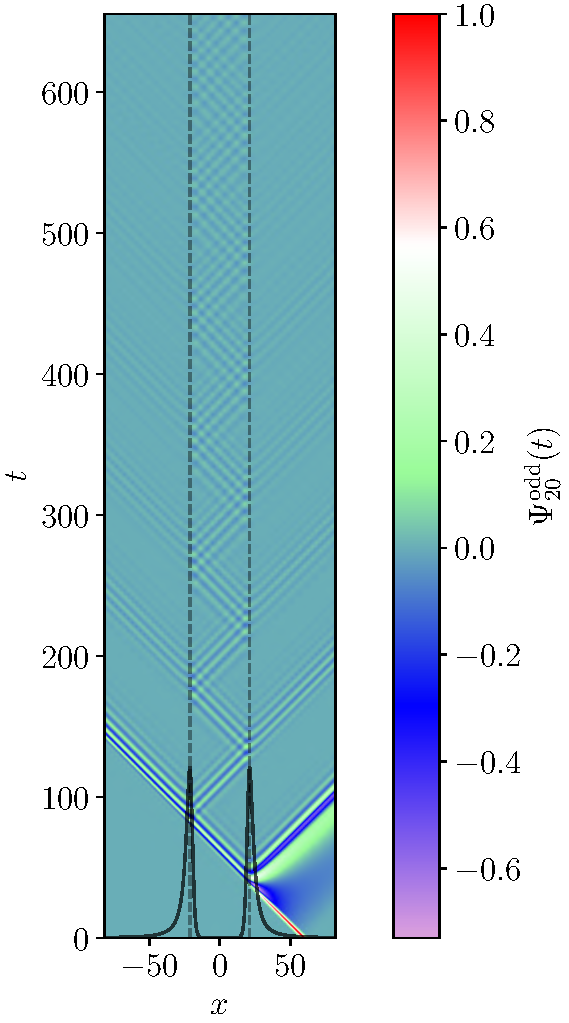
\includegraphics[width=.4\textwidth]{figures/odd_wh_l_2.pdf}
\caption{\label{fig:even_evolve} Evolution of $\Psi^{\mathrm{odd}}$ for an ingoing Gaussian pulse with $\sigma=0.9185r_g$.}
\end{figure}

In Figs.~\ref{fig:odd_sigma_small} and \ref{fig:odd_sigma_large} we see the asymptotic behavior of two solutions with $\sigma=0.9185r_g$ and $\sigma=5.196r_g$, respectively. Observing that the amplitude of the echoes is not large in general, since it varies depending on the spectral content of the initial pulses, which are not the same in the case of initial Gaussian wavelets with different widths.
\par
Frequency dependent reflection and transmission coefficients can be calculated by studying a scattering problem with a single potential wall, as we noticed in subsection \ref{subsec:bh}, this is simply achieved by doing an algebraic inversion of the tortoise coordinate definition in \eqref{eq:tortoise2}: here the inverted function is evaluated in $x-r_g$ instead of $|x|-r_g$. The definition of the reflectivity and transmissivity coefficients is the same as in \eqref{eq:ref_and_trans}

\begin{equation}
R(\omega)\equiv \frac{||\tilde{\Psi}_{\mathrm{ref}}^{\mathrm{odd}}(\omega)||}{||\tilde{\Psi}_{\mathrm{inc}}^{\mathrm{odd}}(\omega)||}~,~T(\omega)\equiv  \frac{||\tilde{\Psi}_{\mathrm{trans}}^{\mathrm{odd}}(\omega)||}{||\tilde{\Psi}_{\mathrm{inc}}^{\mathrm{odd}}(\omega)||},
\label{eq:odd_ref_and_trans}
\end{equation}
where we compute the one dimensional Fourier transforms of the incident $\tilde{\Psi}_{\mathrm{inc}}^{\mathrm{odd}}(\omega)=\mathcal{F}[\Psi^{\mathrm{odd}}_{\mathrm{bh}}(x,0)]$, reflected $\tilde{\Psi}_{\mathrm{ref}}^{\mathrm{odd}}(\omega)=\mathcal{F}[\Psi^{\mathrm{odd}}_{\mathrm{bh}}(+\infty,t)]$ and transmitted $\tilde{\Psi}_{\mathrm{trans}}^{\mathrm{odd}}(\omega)=\mathcal{F}[\Psi^{\mathrm{odd}}_{\mathrm{bh}}(-\infty,t)]$, where the label (bh) stands for the solutions of the scattering problem of \eqref{eq:wave_tensor_wh} with a single potential barrier. These single barrier solutions are not only necessary for the study of the potential cavity, but also to clean up the low frequency (high $\sigma$) solutions, since in those scenarios it is not simple to determine the amplitude of the echoes. Moreover, All of the aforementioned definitions are also applicable for $\Psi^{\mathrm{even}}$. 

\begin{figure}[t!]
\centering
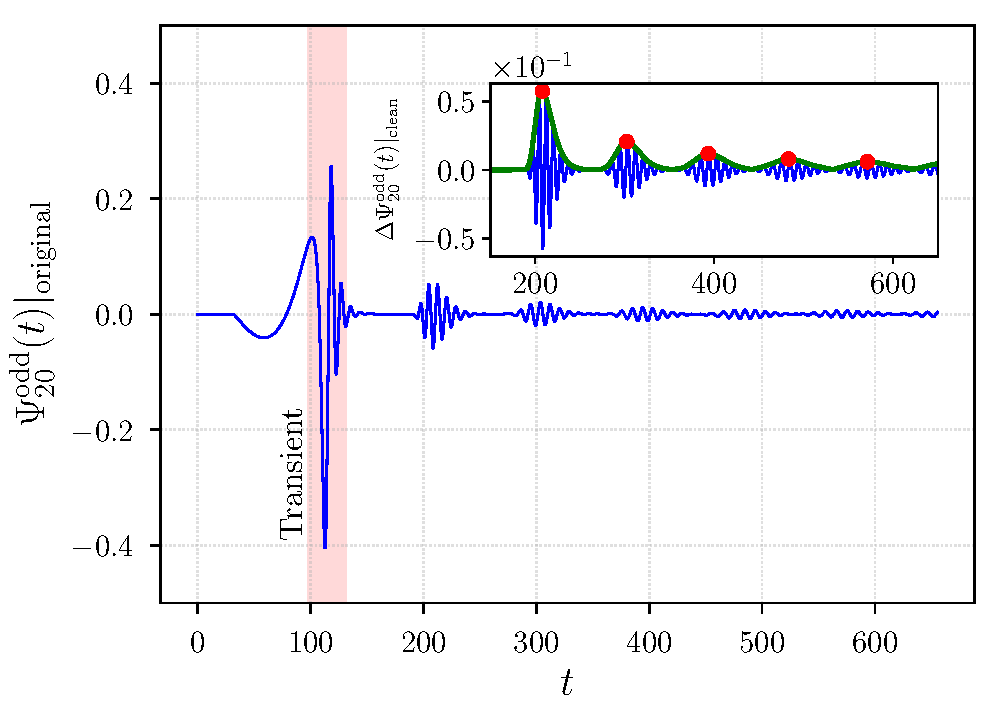
\includegraphics[width=.45\textwidth]{figures/Odd_echo_w_09185.pdf}
\caption{\label{fig:odd_sigma_small} Asymptotic solution of $\Psi^{\mathrm{odd}}_{20}$ considering an incident wavepacket with $\sigma=0.9185r_g$}
\end{figure}

\begin{figure}[t!]
\centering
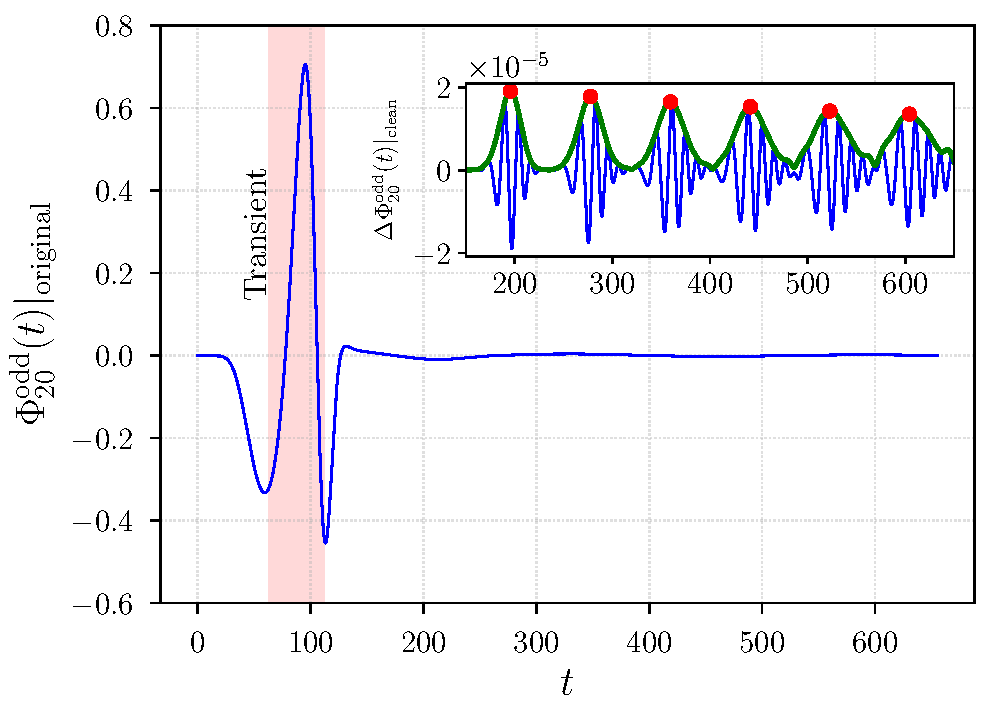
\includegraphics[width=.45\textwidth]{figures/Odd_echo.pdf}
\caption{\label{fig:odd_sigma_large} Asymptotic solution of $\Psi^{\mathrm{odd}}_{20}$ considering an incident wavepacket with $\sigma=5.196r_g$. The amplitude of the echoes is four orders of magnitude smaller than in Fig.~\ref{fig:odd_sigma_large}.}
\end{figure}

In the left panel of Fig.~\ref{fig:RT_reconst}, we show the reflection and transmission coefficients as functions of the frequency, noticing that the two curves intersect at $R^2=T^2=0.5$, as expected. The identity $R^2+T^2$ is approximately satisfied. As a next step of our analysis, we reconstruct the Fourier transform of the asymptotic pulse shown in Fig.~\ref{fig:odd_sigma_small}.  
\begin{figure*}[t!]
\centering
\subfigure{
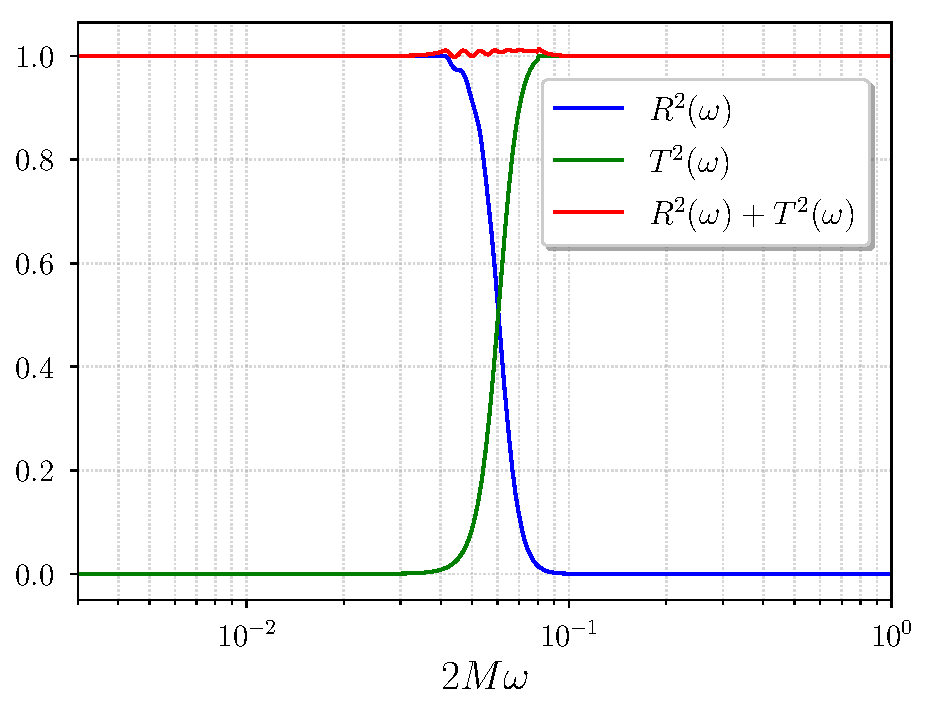
\includegraphics[width=.45\textwidth]{figures/RT_omega_odd.pdf}} \,
\subfigure{
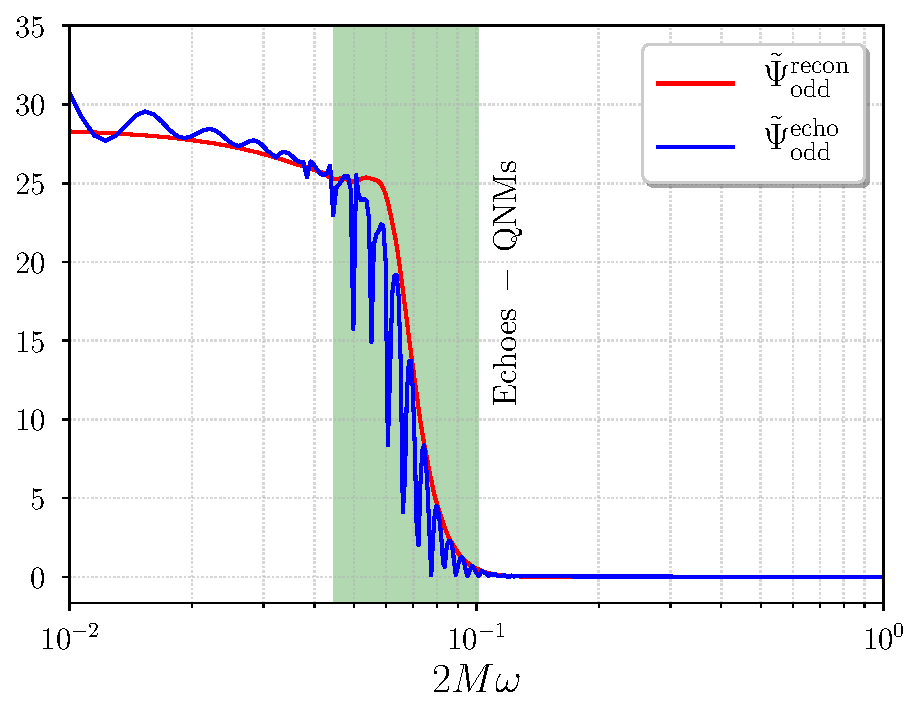
\includegraphics[width=.45\textwidth]{figures/Reconst_omega_odd.pdf}}
\caption{\label{fig:RT_reconst} Left panel: Reflection and transmission coefficients for $\sigma=0.9185r_g$ and the quadrupole $\ell,m=(2,0)$, the ``sweet spot'' in the frequency domain is located around the intersection at $R^2=T^2=0.5$. Right panel: Geometrical optics reconstruction is plotted in red, and it is compared with the Fourier transform of the asymptotic solution shown in Fig.~\ref{fig:odd_sigma_small}. Ignoring the low frequency peaks (introduced by the finite size of the simulation box), we notice that the reconstructed spectrum provides a good idea of the overall shape, but it does not reproduce the power in the frequency of the QNMs. Our results are not dramatically different for the solutions of $\Psi^{\mathrm{even}}$.} 
\end{figure*}
\par
We employed the definition of the geometrical optics approximation in \eqref{eq:reconst}, applied up to $i=0$, in the Fourier transform of the Gaussian incident wavepacket in order to obtain the reconstructed profile in the right panel of Fig.~\ref{fig:RT_reconst}. The signal reconstructed using the geometrical optics approximation provides a better representation of the total reflected pulse as the ingoing wavelet gets wider, and therefore, it has more power in lower frequencies. 

Motivated by the drastic change in the amplitudes of the echoes seen in Figs.~\ref{fig:odd_sigma_small} and \ref{fig:odd_sigma_large}. We now explore the dependence of the amplitude of each individual echo with the width of the incident Gaussian pulse. To do so, we follow the same procedure explained by the end of subsection \ref{subsec:wh}: we construct a logarithmic grid in $\sigma$, centered at $\sigma_{\mathrm{DW}}=\sqrt{27}r_g/2\ell$ and spaced in intervals of $\sqrt{2}\sigma_{\mathrm{DW}}$. In addition to this, we define the variable $\Delta\Psi^{\mathrm{odd}}_{\mathrm{clean}}\equiv\Psi^{\mathrm{odd}}_{\mathrm{original}}-\Psi^{\mathrm{odd}}_{\mathrm{bh}}$ in order to clean the solutions from backscattering effects coming from the potential tails, which complicate the task of determining the amplitudes of the echoes with high $\sigma$/low frequency. Once the solutions are clean, the most effective way to find the maxima of each echo is by calculating the local maxima of the Hilbert envelope for the clean signal. In this case, the Hilbert envelopes are the green curves in the upper corner of Figs.~\ref{fig:odd_sigma_small} and \ref{fig:odd_sigma_large} and the maxima are the red dots on top of each curve. 
This labor is even more computationally expensive than the scalar case, not only because we are solving the scattering problem for two systems: one with a potential barrier and another with the potential cavity; but also we are now working with the two polarizations (i.e., the even and odd solutions). Our results of the amplitude analysis in Fig.~\ref{fig:echo_sigma_odd}, showing the existence of a value of $\sigma$ maximizing the amplitude of the echoes. This is compatible with the notion of a band of widths/frequencies in which the echoes have sufficient amplitude to be measured.    

\begin{figure*}
\centering
\subfigure{
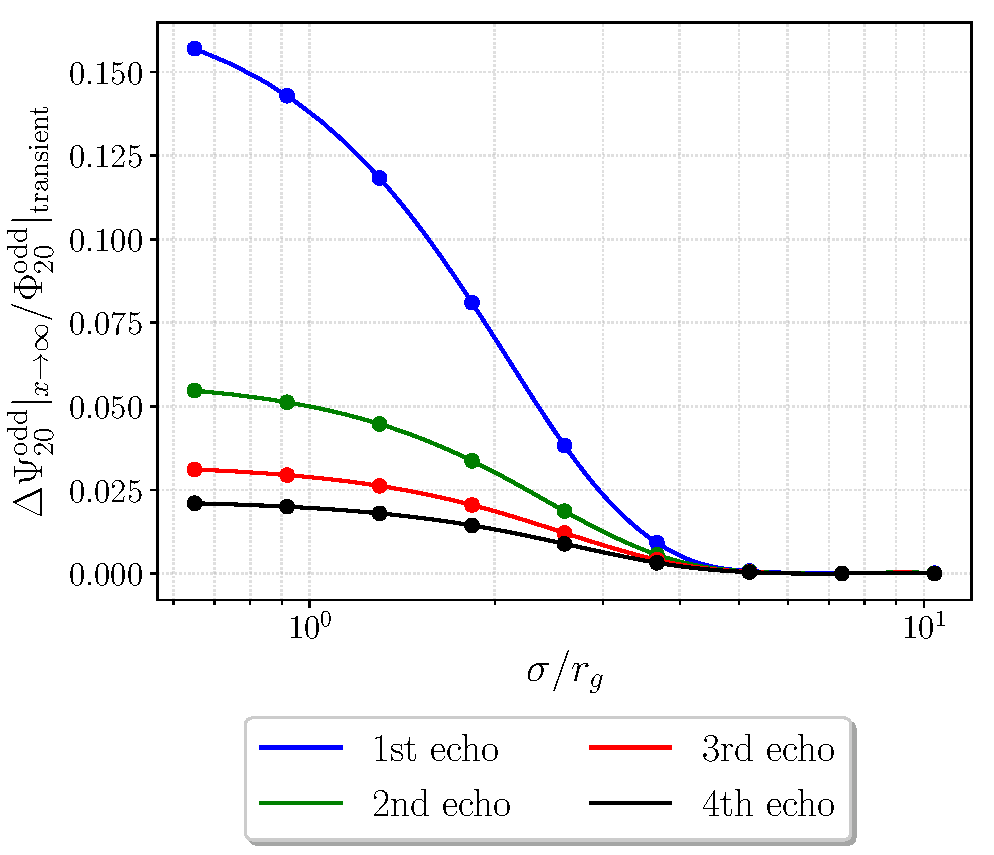
\includegraphics[width=.45\textwidth]{figures/Echo_sigma_odd_l_2.pdf}} \,
\subfigure{
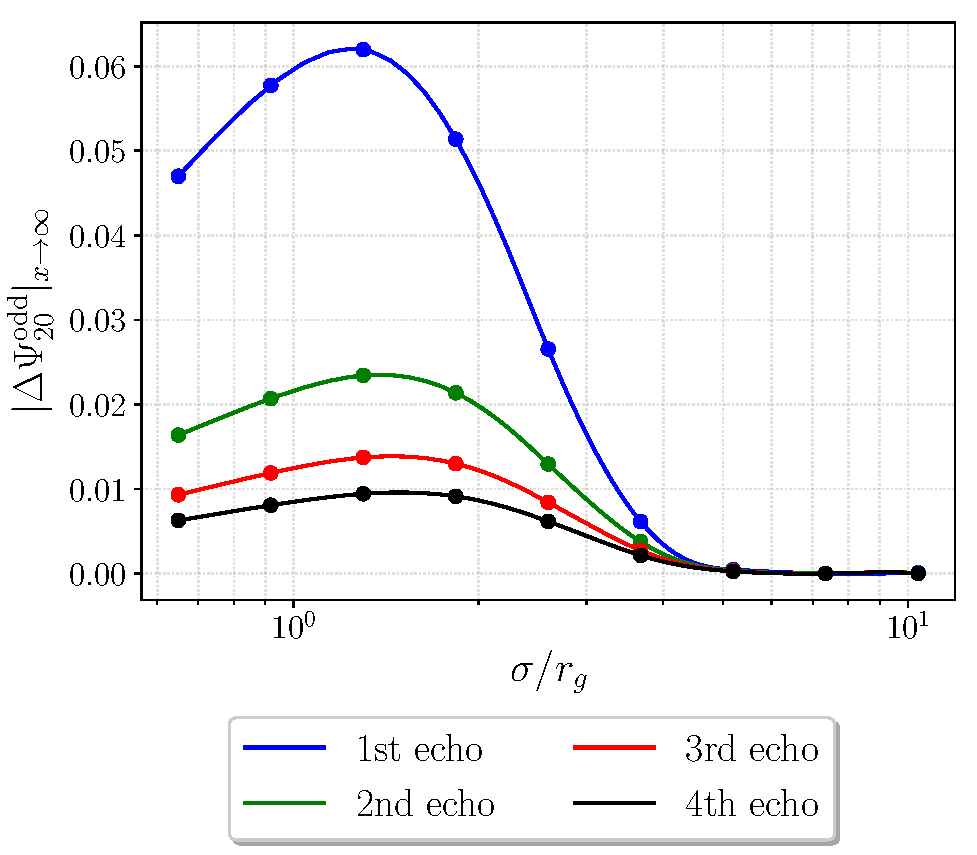
\includegraphics[width=.45\textwidth]{figures/Echo_sigma2_odd_l_2.pdf}} 
\caption{\label{fig:echo_sigma_odd} Left panel: Amplitudes of the first four echoes of $\Psi^{\mathrm{odd}}_{20}$ as a function of $\sigma$ for $\ell=2$. Right panel: Relative amplitude of the first four echoes compared to the amplitude of the transient. The points represent the simulated double/single wall pairs used in our analysis, as in Fig.~\ref{fig:echo_sigma}. These results are not significantly different for $\Psi^{\mathrm{even}}_{20}$.} 
\end{figure*}
\section{Conclusions}\label{sec:conclusions}
In this paper, we studied the scattering of a test scalar and tensor wavepacket on a wormhole. Using a Gaussian wavelet as an incident initial condition, we showed the time dependent scattering solution of the quadrupole scalar and tensor spherical modes both inside and outside the potential cavities in Figs.~\ref{fig:sol_n_flux_wh} and \ref{fig:even_evolve}. Furthermore, after finding the transmission and reflection coefficients of the cavities in Fig.~\ref{fig:RT_scalar} and in the left panel of Fig..~\ref{fig:RT_reconst}, we used the geometrical optics approximation to reconstruct the shape of the Fourier transformed asymptotic solutions in Fig.~\ref{fig:rec_scalar} and in the right panel of Fig.~\ref{fig:RT_reconst}. Finding that the reconstruction is accurate up to the quasinormal mode peaks, which were also identified in the spectrum along with the span of frequencies where these can be found. 

We found that in general, the echoes do not have a large amplitude as we can see directly in the left panel of Fig.~\ref{fig:asympt_two_sigmas} and in Fig.~\ref{fig:odd_sigma_large}. Moreover, there is a band of preferred frequencies and widths that maximizes the amplitude of the echoes. The frequency band is centered around the ``sweet spot'' in which the coefficients of transmissivity and reflectivity overlap, and it is precisely where the QNMs peaks are squeezed in. We extended our analysis to find the range in which the incident width of the incident pulse maximizes the amplitude of the first four echoes, and how large is their amplitude compared to the transient. In Figs.~\ref{fig:echo_sigma_odd} and \ref{fig:echo_sigma}, we found that for low widths of the ingoing signal, as the widths become smaller, the transient decreases faster than the amplitude of the echoes. 
\begin{figure}[t!]
\centering
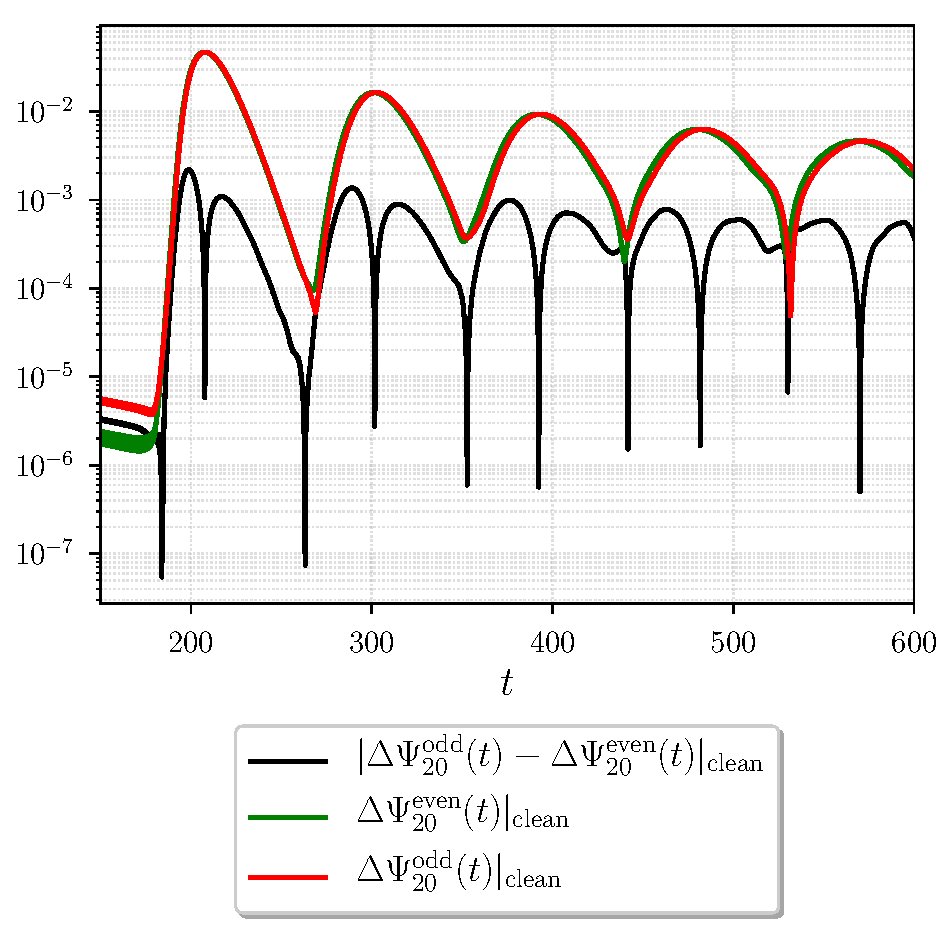
\includegraphics[width=.45\textwidth]{figures/Polarimetry_echo_w_06495.pdf}
\caption{\label{fig:pol} Comparing the Hilbert envelopes of the two clean solutions for echoes. We can see a very small excess in amplitude coming from the odd solution, which means that the outgoing signal might have a small net polarization even in the scenario of an incident test Gaussian wavepacket of tensor perturbations with no preferred polarization.}
\end{figure}

\appendix
\section{Echoes and gravitational wave polarimetry}
\label{sec:AppendixPolar}


The small difference in the even and odd potentials is shown in the right panel of Fig.~\ref{fig:evenodd_potentials} has an effect. In order to illustrate it, we will just work with the even and odd quadrupole signals in the equatorial plane. In the case of a generic spherical mode with equal contributions from $\Psi^{\mathrm{odd}}_{20}$ and $\Psi^{\mathrm{even}}_{20} $, which are the first nontrivial contributions to \eqref{eq:hplus} and \eqref{eq:hx}, we notice that the two polarizations have the form 


\begin{eqnarray}
h_+(x,t)=\frac{C_1}{r(|x|)}\Psi^{\mathrm{even}}_{20}(x,t),\nonumber\\
h_{\times}(x,t)=\frac{C_2}{r(|x|)}\Psi^{\mathrm{odd}}_{20}(x,t),\label{eq:pols}
\end{eqnarray}
where $C_1$ and $C_2$ are constants coming from the angular dependence. Therefore, the existence of echoes might generate a slightly polarized wave, as we can see from Fig.~\ref{fig:pol}. It is interesting to notice these effects in a spherically symmetric system even when these are tiny. Kerr-like solutions might increase the polarization effects.
    
\begin{acknowledgments}
We would like to thank Alex Zucca, Levon Pogosian and Michael Desrochers for their time and their valuable comments and discussions. This project was partly funded by the Discovery Grants program of the Natural Sciences and Engineering Research Council of Canada. JG is supported by the Billy Jones Graduate Scholarship, granted by the Physics Department at SFU. This research was enabled in part by support provided by WestGrid (\url{www.westgrid.ca}) and Compute Canada Calcul Canada (\url{www.computecanada.ca})
\end{acknowledgments}
\bibliography{bibliography.bib}

\end{document}
